%!TEX root = ../rapport.tex
%!TEX encoding = UTF-8 Unicode
% Chapitres "Annexes"

% modifié par Francis Valois, Université Laval
% 31/01/2011 - version 1.0 - Création du document
\chapter{Projet 1}
\label{s:annexes}
Les courbes présentées dans cet annexe sont présentées à titre formatif. Ces courbes nous ont aidé à mieux saisir l'impact d'une mauvaise adaptation de la charge sur les réflexions vues à la source.
\begin{figure}[htb]
	\centering
\subfigure[Courbes de réflexion obtenue pour $R = 0\Omega$]{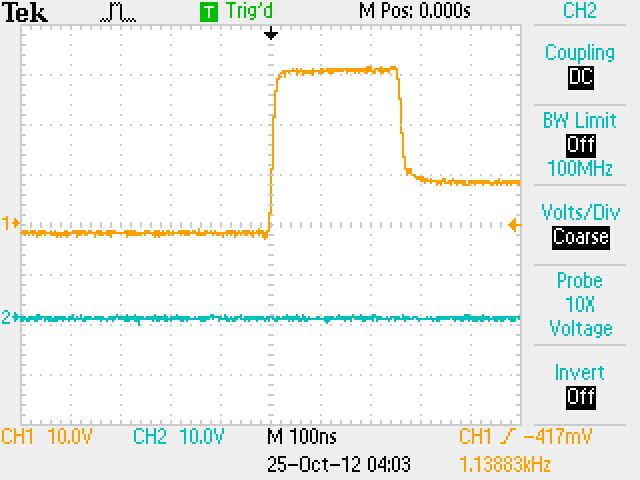
\includegraphics[scale =0.3]{fig/RR0.JPG} \label{fig:reflexr0}}
		\quad
		\subfigure[Courbes de réflexion obtenue pour $R = 27\Omega$]{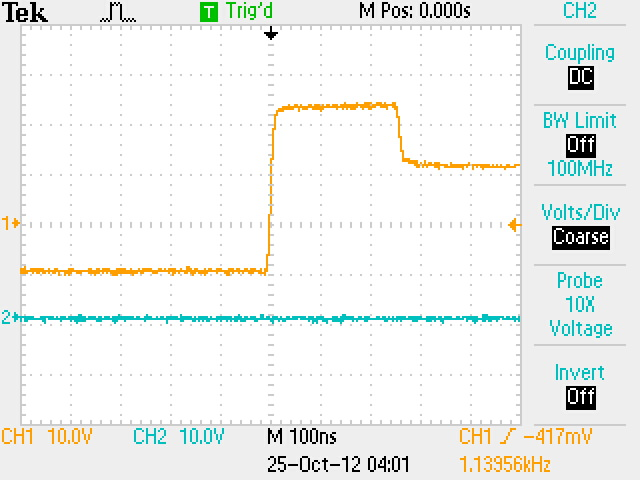
\includegraphics[scale =0.3]{fig/RR27.JPG} \label{fig:reflexr27}}
		\quad
		\subfigure[Courbes de réflexion obtenue pour $R = 50\Omega$]{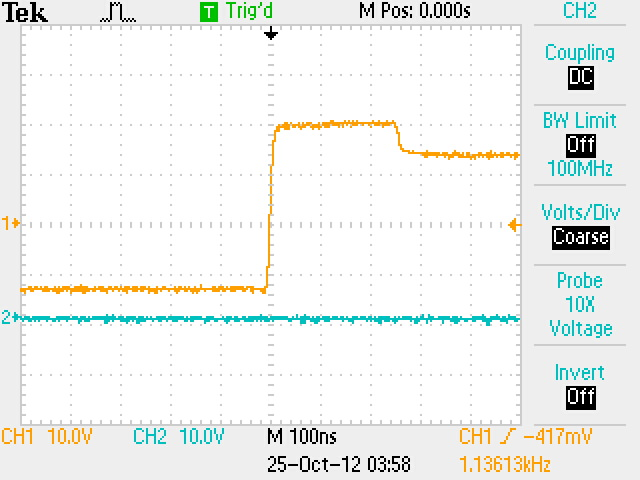
\includegraphics[scale =0.3]{fig/RR50.JPG} \label{fig:reflexr50}}
		\quad
		\subfigure[Courbes de réflexion obtenue pour $R = \infty$]{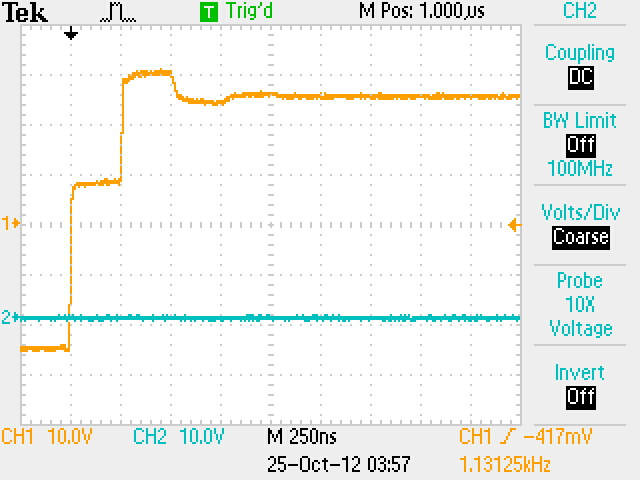
\includegraphics[scale =0.3]{fig/RRCO.JPG} \label{fig:reflexrco}}
\end{figure}


